\subsection{IBD for PC}

På figur \ref{fig:ibd_pc} ses alle interne signaler og en yderligere specificering af blokdiagrammet for pc på figur \ref{fig:bdd_pc}

\begin{figure}[h]
\centering
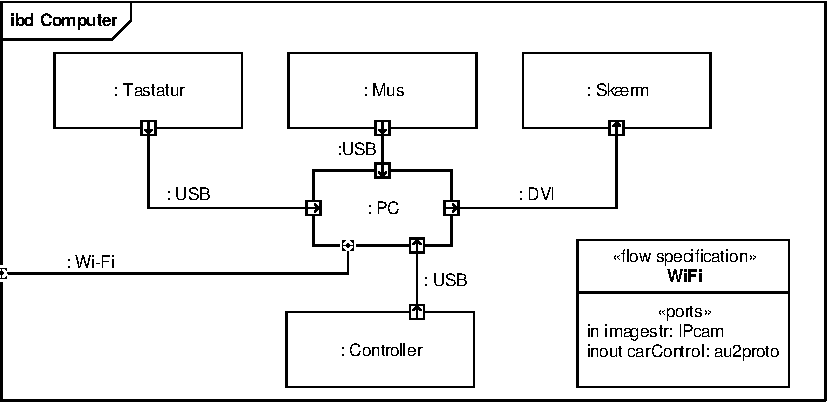
\includegraphics[scale=1]{../fig/diagrammer/pc/ibd_pc.pdf}
\caption{IBD for blokken PC}
\label{fig:ibd_pc}
\end{figure}

\subsection{Signalbeskrivelse for PC}

\begin{table}[h]
	\centering
	\begin{tabularx}{\textwidth}{|l|X|X|X|} \hline
	\textbf{Signal (navn: type)} & \textbf{Funktion} & \textbf{Tolerancer} & \textbf{Kommentarer} \\ \hline
Imagestr: IPcam
	& TODO Karsten %TODO Karsten
	& 
 	& 
	\\ \hline
	
carControl: au2proto
	& TODO Karsten %TODO Karsten
	& 
	& 
	\\ \hline
	
Tastetur: USB
	& Serielkommunikation fra tastetur til PC 
	& VBUS = 5V min. 4.40V max 5.25V \newline
		GND = 0V \newline
		D- = 5V +/- 0.2V \newline
		D+ = 5V +/- 0.2V \newline
	
	& VBUS for Low power port: \newline
		Diff  “1” \newline
		(D+) - (D-) > 200 mV \newline
		and D+ > VIH (min) \newline
		Diff ”0” \newline
		(D-) - (D+) > 200 mV \newline
		and D- > VIH (min) \newline
	
	\\ \hline	
	
Mus: USB
	& Serielkommunikation fra mus til PC 
	& VBUS = 5V min. 4.40V max 5.25V \newline
		GND = 0V \newline
		D- = 5V +/- 0.2V \newline
		D+ = 5V +/- 0.2V \newline

	& VBUS for Low power port: \newline
		Diff  “1” \newline
		(D+) - (D-) > 200 mV \newline
		and D+ > VIH (min) \newline
		Diff ”0” \newline
		(D-) - (D+) > 200 mV \newline
		and D- > VIH (min) \newline

\\ \hline
	
displayConn:
	&   
	&  
	&  
	\\ \hline
	
Controller: USB
	& Serielkommunikation fra Controller til PC 
	& VBUS = 5V min. 4.40V max 5.25V \newline
		GND = 0V \newline
		D- = 5V +/- 0.2V \newline
		D+ = 5V +/- 0.2V \newline
	& VBUS for Low power port: \newline
		Diff  “1” \newline
		(D+) - (D-) > 200 mV \newline
		and D+ > VIH (min) \newline
		Diff ”0” \newline
		(D-) - (D+) > 200 mV \newline
		and D- > VIH (min) \newline
	\\ \hline
	
	\end{tabularx}
\end{table}